\documentclass[12pt]{article}

\usepackage[
    a4paper,
    hmargin=2cm, vmargin=1.3cm,
    headheight=56.6pt, % as per the warning by fancyhdr
    headsep=10pt,
    includehead, includefoot
]{geometry}

\usepackage[english]{babel}
\usepackage[T1]{fontenc}
\usepackage[utf8x]{inputenc}

\usepackage{fancyhdr} % extensice control of page headers and footers
\usepackage{graphicx}
\usepackage{parskip} % add space between paragraphs and remove first line's indent

\usepackage[dvipsnames,table]{xcolor} % color the text for the color code: https://en.wikibooks.org/wiki/LaTeX/Colors
\usepackage[bottom]{footmisc} % to place footnotes to the bottom of the page
% \usepackage{pdfpages} % \includepdf[pages=-]{myfile.pdf}: all pages, or `pages={1}`
\usepackage{amsmath} % provides math environments
\usepackage{amssymb} % add math symbols
\usepackage{cancel} % https://tex.stackexchange.com/a/75530/164820
\usepackage{ifthen} % provides \ifthenelse test
\usepackage{xifthen} % provides \isempty test
\usepackage{float} % improve the figure placement in the document
\usepackage[normalem]{ulem} % used to strike through: https://jansoehlke.com/2010/06/strikethrough-in-latex/
\usepackage{multirow}
\usepackage{hhline} % https://tex.stackexchange.com/a/39766/164820
\usepackage[acronym,nonumberlist,nogroupskip]{glossaries} % to handle acronyms

% Fix non breakable links: https://tex.stackexchange.com/a/3034/164820
\PassOptionsToPackage{hyphens}{url}\usepackage{hyperref}
\usepackage[inline]{enumitem} % allow to set some margin to list env's
\usepackage{tcolorbox}

\usepackage{listings}
\usepackage{tikz}
\usetikzlibrary{calc}
\usepackage{pgfplots}


% ---------------- SETUP HEADER & FOOTER ----------------------
\pagestyle{fancy}
% \fancyhf{} % sets both header and footer to nothing
% \renewcommand{\headrulewidth}{0pt} % remove headers bottom line


% Define variables
\makeatletter
\newcommand{\prof}[1]{\def\@prof{#1}}
\newcommand{\theprof}{\@ifundefined{@prof}{}{\\Prof.: \@prof}}
\newcommand{\student}[1]{\def\@student{#1}}
\newcommand{\thestudent}{\@ifundefined{@student}{}{\@student}}
\newcommand{\seriesnumber}[1]{\def\@seriesnumber{#1}}
\newcommand{\theseriesnumber}{\@ifundefined{@seriesnumber}{}{Series \@seriesnumber}}
\makeatother


% https://tex.stackexchange.com/a/218450/164820
\lstnewenvironment{algorithm}[1][] %defines the algorithm listing environment
{
    % \refstepcounter{nalg} %increments algorithm number
    % \captionsetup{labelformat=algocaption,labelsep=colon} %defines the caption setup for: it ises label format as the declared caption label above and makes label and caption text to be separated by a ':'
    \lstset{ %this is the stype
        mathescape=true,
        frame=tB,
        numberstyle=\tiny,
        basicstyle=\scriptsize,
        keywordstyle=\color{black}\bfseries\em,
        keywords={,input, output, return, datatype, initialize, do, function, in, if, else, then, foreach, break, while, begin, end} %add the keywords you want, or load a language as Rubens explains in his comment above.
        % numbers=left,
        xleftmargin=.04\textwidth,
        #1 % this is to add specific settings to an usage of this environment (for instnce, the caption and referable label)
    }
}
{}



\newcommand{\unilogo}[1][0.16\textwidth]{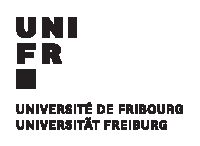
\includegraphics[width=#1]{logo_uni}}

\newcommand*{\fullref}[1]{\hyperref[{#1}]{\autoref*{#1}} \textit{\nameref*{#1}}} % https://tex.stackexchange.com/a/121871
\newcommand*{\simpleref}[1]{\hyperref[{#1}]{{\autoref*{#1}}}}
\newcommand*{\namedref}[2]{\hyperref[{#1}]{\textit{#2}}}
\newcommand*{\visitedurl}[2]{\url{#1}\hspace{0.6em}(visited on #2)}
\newcommand*{\footnotelink}[2]{\footnote{\visitedurl{#1}{#2}}}
\newcommand*{\footnotetextlink}[2]{\footnotetext{\visitedurl{#1}{#2}}}

\newcommand*{\notice}[2][Notice]{
Notice:
\begin{itemize}
    \vspace{-0.2cm}
    \item #2
\end{itemize}
}


\newcommand{\yellowInBlue}[1]{{\colorbox{blue!50}{\color{yellow}\textbf{#1}}}}

\newcommand*{\todo}[1]{
    \ifthenelse{\isempty{#1}}
        {\yellowInBlue{TODO}}
        {\yellowInBlue{TODO #1}} % else
}



\newcounter{question}[section]
\newcommand{\questioncolor}{\color{CadetBlue}}
\def\newquestion#1{
    \refstepcounter{question}
    {
        \textbf{Question~\arabic{question}.}
        \questioncolor
        \emph{#1}
    }
}
\def\question#1{
    {
        \questioncolor
        \emph{#1}
    }
}


\setlist[description]{leftmargin=0.5cm,labelindent=0.5cm,parsep=0.4ex}

% Table layout
\def\arraystretch{1.5} % height of each row is set to 1.5 relative to its default height.
\setlength{\tabcolsep}{8pt} % space between the text and the left/right border

\glsenablehyper
\hypersetup{
	colorlinks = true,
	% linkcolor = red,
	% menucolor = red,
	% filecolor = blue,
	% anchorcolor = green,
	% urlcolor = blue,
	allcolors = MidnightBlue,
	linkbordercolor = white
}

\definecolor{commentcolor}{HTML}{969896}
\definecolor{mGray}{rgb}{0.5,0.5,0.5}
\definecolor{stringcolor}{HTML}{769107}
\lstset{
    % language=csh,
    % numbers=left,
    % numbersep=5pt,
    % numberstyle=\tiny,
    aboveskip=12pt,
    basicstyle=\linespread{1.05}\small\ttfamily,
    belowskip=9pt,
    breaklines=true,
    captionpos=b,
    commentstyle=\color{commentcolor},
    extendedchars=true,
    frame=tb,
    framexbottommargin=4pt,
    framexleftmargin=17pt,
    framexrightmargin=5pt,
    keywordstyle=\color{magenta},
    numbers=none,  % still add them: numbers=left
    numberstyle=\tiny\color{mGray},
    showspaces=false,
    showstringspaces=false,
    showtabs=false,
    stringstyle=\color{stringcolor}\ttfamily,
    tabsize=2,
    xleftmargin=17pt,
}

\loadglsentries{../glossary}
\makeglossaries


\graphicspath{{../assets/}}


\title{
    %\vspace{-2cm}
    \unilogo[0.3\textwidth]\\[0.9cm]
    S07: Data Structure
}
\student{
    A. Schaller\\
    \texttt{16-896-375}
}
\prof{Dr. Luggen Michael}

\seriesnumber{7}
\author{\thestudent\theprof}
\lhead{\unilogo}
\rhead{\thestudent\\\theseriesnumber}

% \usepackage[backend=bibtex, style=numeric, citestyle=numeric, sorting=none, backref, backrefstyle=none]{biblatex}
% use "biber report" command to generate

% \addbibresource{biblio.bib}


% \usepgfplotslibrary{fillbetween}
\pgfplotsset{compat=newest}
% \usepackage{fontawesome}

\lstset{
    language=C,
    basicstyle=\footnotesize,
    stepnumber=3,
    firstnumber=1,
}

\raggedbottom % To avoid stretching the items to fill a page
% ---------------------- DOCUMENT ----------------------------
\begin{document}

\maketitle

%
%
% ---------------------------------
\section{Some Linked List Data Structures}

\newquestion{Using struct, declare the data structure of the following structures:}

\begin{enumerate}[label={\questioncolor\arabic*.}]
    \item \question{a linked list}

\begin{lstlisting}
struct node {
    int data;
    struct node * next;
};
\end{lstlisting}

    Or replace the \verb!int data! with the type expected to be in the structure, or replace it with a pointer, which will be using the same amount of memory to point to any data.


    \item \question{a doubly linked list}

\begin{lstlisting}
struct node {
    int data;
    struct node * previous;
    struct node * next;
};
\end{lstlisting}

    \textit{Same comment as the previous linked list.}

    \item \question{a linked binary tree}

\begin{lstlisting}
struct node {
    int data;
    struct node * left;
    struct node * right;
};
\end{lstlisting}

    \textit{Same comment}.

\end{enumerate}




%
%
% ---------------------------------
\section{Pointer Manipulation}

\newquestion{Define a data structure that corresponds to the sketch in \namedref{fig:fig1}{Fig.1.}, and implement the function void swap\_ptr() allowing to swap the two top elements as showed in \namedref{fig:fig1}{Fig.1.}.}

{\color{gray} \textbf{Remark} -- To simplify the implementation of swap\_ptr(), we
assume that the data structure contains at least 2 nodes, i.e. no error
checking has to be performed. Beware that your solution should also work
when the structure contains only 2 nodes.}


\begin{figure}[H]
    \center
    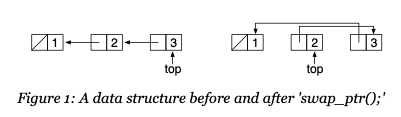
\includegraphics[width=0.7\textwidth]{s07/swap_ptr.png}
    \label{fig:fig1}
\end{figure}


The \namedref{fig:fig1}{Fig.1.} represent a \emph{simple linked list} and the swap operation is equivalent to swapping the payload of the head with its previous node's payload (even though the name isn't really representative of the behavior).

\begin{lstlisting}
struct node {
    int data;
    struct node * next;
};

void swap_ptr(struct node * head) {
    int headData = head->data;
    int nextData = head->next->data;

    head->data = nextData;
    head->next->data = headData;
}
\end{lstlisting}

%
%
% ---------------------------------
\section{Queue}

\newquestion{Study the \href{https://unifr.coursc.ch/7/linked_list_stack.c}{linked\_list\_stack.c}\footnotelink{https://unifr.coursc.ch/7/linked_list_stack.c}{April 2021}
source code and transform it to implement a queue. A queue is a data
structure in which objects are accessed in FIFO (First In First Out)
order. New objects are inserted at the end of the queue (enqueue).
Object is removed from the beginning (dequeue).}

{\color{gray}\textbf{Hint} -- to easily access the end of the queue, you need to store
an additional pointer to the last element of your linked list. Create a
structure struct Queue which will store the head node and tail node of
the list.}


\begin{figure}[H]
    \center
    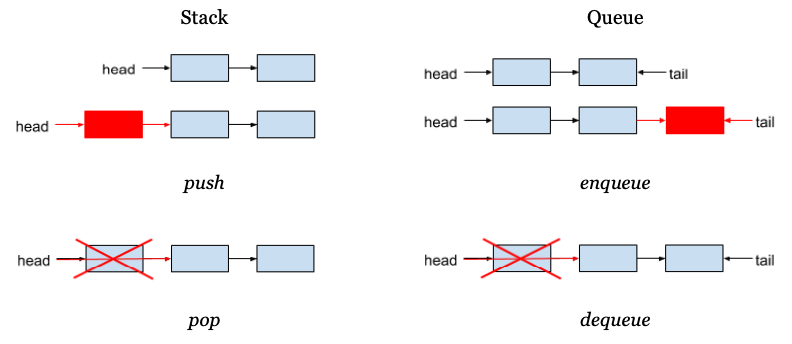
\includegraphics[width=0.9\textwidth]{s07/stack_queue}
    \label{fig:stack_queue}
\end{figure}


\begin{lstlisting}{caption={Naive implementation of a Queue}}
#include <stdio.h>
#include <stdlib.h>

struct Node {
    int data;
    struct Node * next;
};

struct Queue {
    struct Node * head;
    struct Node * tail;
};

void printLinkedlist(struct Node * p);

void enqueue (struct Queue * q, struct Node * newTail) {
    if (q->tail) {
        q->tail->next = newTail;
    }
    // if we don't have a tail, we neither have a head, unless external
    // change
    else {
        q->head = newTail;
    }

    // If we allow enqueuing a tail with multiple nodes, then we have
    // to look for the deepst tail
    // -- Possible improvement? --
    q->tail = newTail;
}

void enqueue_value (struct Queue * q, int value) {
    struct Node * newNode = malloc(sizeof(newNode));
    newNode->data = value;
    enqueue(q, newNode);
}

struct Node * dequeue (struct Queue * q) {
    struct Node * head = q->head;

    if (head) {
        q->head = head->next;
        head->next = 0;
    }

    return head;
}

int main () {
    struct Queue * q = malloc(sizeof(q));
    enqueue_value(q, 2);
    enqueue_value(q, 5);
    enqueue_value(q, 10);

    printLinkedlist(q->head);

    struct Node * node = dequeue(q);
    printf("Dequeued element: %d (next: %p)\n", node->data, node->next);

    struct Node last = { 15, 0 };
    enqueue(q, &last);

    printLinkedlist(q->head);
}
\end{lstlisting}


%
%
% ---------------------------------
\section{Graph}

\newquestion{Study the
\href{https://unifr.coursc.ch/7/minimal_tree.c}{minimal\_tree.c}\footnotelink{https://unifr.coursc.ch/7/minimal_tree.c}{April 2021} source
code. Suggest a new data structure to be able to express directed graphs
instead of trees:}


\begin{itemize}
    \item \question{Modify the struct node structure and the newNode function.}

\begin{lstlisting}
// 1. modifiy the struct
struct LinkedNode {
    struct GraphNode * target;
    struct LinkedNode * next;
};

struct GraphNode {
    int data;
    struct LinkedNode * directed_relations;
};

// 2. modifiy the newNode function
struct GraphNode * new_graph_node (int data) {
    struct GraphNode * newNode = malloc(sizeof(newNode));
    newNode->data = data;
    newNode->directed_relations = 0;
    return newNode;
}
\end{lstlisting}

    \item \question{Write an additional function connect which allows to connect two arbitrary nodes in your graph.}

\begin{lstlisting}
struct LinkedNode * new_linked_node (struct GraphNode * g) {
    struct LinkedNode * newNode = malloc(sizeof(newNode));
    newNode->target = g;
    newNode->next = 0;
    return newNode;
}

void connect (struct GraphNode * source, struct GraphNode * target) {
    // should maybe also check if the target is not in the directed_relations list
    struct LinkedNode * last_relation = source->directed_relations;
    struct LinkedNode * new_relation_target = new_linked_node(target);
    if (last_relation) {
        while (last_relation->next) {
            last_relation = last_relation->next;
        }

        last_relation->next = new_relation_target;
    }
    // no directed_relations yet
    else {
        source->directed_relations = new_relation_target;
    }
}
\end{lstlisting}


\end{itemize}

A running example using those different structures and functions:
\begin{lstlisting}
void print_relations (struct GraphNode * node) {
    int data = node->data;
    printf("%d", data);
    if ( ! node->directed_relations) {
        // has no directed relation
        printf(" has no directed relations\n");
    }

    struct LinkedNode * r = node->directed_relations;
    printf(" relations:");
    while (r) {
        printf(" %d", r->target->data);
        r = r->next;
    }
    printf("\n");
}

/*
* Example graph to build:
*
*              5
*            / |
*           /  |
*          /   |
*         v    v
*         2-+  1  +-->4
*         \ +--+--+ / ^
*          \   |   / /
*           \  |  / /
*            \ | / /
*             vvv /
*              3
*/

int main () {
    struct GraphNode * top = new_graph_node(5);
    struct GraphNode * left = new_graph_node(2);
    struct GraphNode * middle = new_graph_node(1);
    struct GraphNode * right = new_graph_node(4);
    struct GraphNode * bottom = new_graph_node(3);

    connect(top, left);
    connect(top, middle);

    connect(left, right);
    connect(left, bottom);

    connect(middle, bottom);

    connect(right, bottom);

    connect(bottom, right);

    print_relations(top);
    print_relations(left);
    print_relations(middle);
    print_relations(right);
    print_relations(bottom);
}
\end{lstlisting}

And its output:

\begin{lstlisting}[language={}]
5 relations: 2 1
2 relations: 4 3
1 relations: 3
4 relations: 3
3 relations: 4
\end{lstlisting}



%
%
% ---------------------------------
\section{Project P01: Linked Data In-Memory Store}

\newquestion{Think about the data structure you want to use for your storage. Describe it, its advantages and potential pitfalls.}


\end{document}